Diferentemente de problemas de otimização escalar, problemas multiobjetivo
envolvem a otimização simultânea de múltiplas de funções objetivo geralmente
conflitantes entre si.
Estes problemas não possuem tipicamente uma única solução, mas um conjunto
de soluções de interesse chamado \emph{\paretoset{}}.
Este conjunto é formado pelas soluções ditas \emph{não dominadas} ou \emph{eficientes},
para as quais não é possível melhorar um dos valores de objetivo sem degradar um outro.

Dentre os problemas multiobjetivo bastante estudados
está o problema da mochila multiobjetivo.
Semelhantemente ao problema da mochila $0-1$ clássico,
uma instância do problema da mochila multiobjetivo consiste de um conjunto
de itens possuindo cada um deles um determinado peso,
dos quais deve-se selecionar um subconjunto, cujos pesos somados não excedam uma
capacidade definida.
Porém, diferentemente do caso clássico, cada item selecionado contribui
simultaneamente para múltiplos objetivos, os quais se deseja maximizar.

%Diversos problemas reais podem ser modelados como uma instância deste problema,
%tais como seleção de projetos~\cite{teng1996multiobjective},
%orçamento de capital~\cite{rosenblatt1989generating},
%planejamento~\cite{jenkins2002bicriteria}
%e planejamento de estoque~\cite{ishibuchi2015behavior}.
%Este problema tem despertado o interesse de vários pesquisadores e vários
%métodos de resolução, tanto exatos quanto heurísticos, tem sido propostos.

Diversos problemas reais podem ser modelados como uma instância do problema da mochila multiobjetivo.
Um deles é o problema de seleção de projeto~\cite{teng1996multiobjective}.
Nele deseja-se selecionar, dentre um portfolio definido de projetos,
um subconjunto para ser executado considerando um orçamento limitado.
A execução de cada um dos projetos beneficia múltiplos critérios como,
por exemplo, múltiplas partes interessadas.
Deseja-se então determinar o subconjunto que maximiza simultaneamente a contribuição total
para cada critério estabelecido, o que caracteriza um problema multiobjetivo.

Outro problema que pode ser modelado como um problema da mochila multiobjetivo
é o problema de orçamento de capital com risco~\cite{rosenblatt1989generating}.
Nesse problema, considera-se um conjunto de investimentos,
do qual deseja-se selecionar um subconjunto para ser executado, dado um orçamento limitado.
Cada investimento possui um valor de lucro e também um fator de risco (ou variância) associado,
fazendo com que a seleção de um subconjunto de investimentos configure, não apenas um lucro total,
mas também um valor de risco associado total.
A escolha do melhor subconjunto de investimentos depende de uma soma ponderada do lucro total
ao risco total acumulado.
Porém, o fator de ponderação, que representa a vantagem do lucro sobre o risco,
não é previamente conhecido, mas determinado em um momento posterior.
Por esse motivo, a etapa de solução do problema deve considerar
a maximização simultânea do lucro e do fator risco acumulado,
o que caracteriza o problema multiobjetivo.

Em~\cite{jenkins2002bicriteria} o problema da mochila multiobjetivo é
utilizado para modelar um problema de planejamento de ações para remediar
poluição em porções terrestres.
Nesse problema, deseja-se planejar a execução de ações de remoção de poluição
para tratar diversos postos de guarda marítima.
Essas ações não serão aplicadas em todos os postos simultaneamente,
mas separadas em duas fases, sendo que
para a primeira existe um orçamento limitado.
Após uma avaliação preliminar dos postos quanto ao nível de poluição,
um quadro de ações é estabelecido para cada posto.
A partir de então, deve-se decidir, quais postos serão tratados
imediatamente (primeira fase) e quais serão tratados posteriormente (segunda fase).
Para cada posto, a aplicação imediata das ações provê dois critérios de retribuição:
(a) uma pontuação junto ao respectivo órgão ambiental e
(b) uma métrica associada à estimativa de incompletude da avaliação preliminar do posto.
O objetivo do problema é definir, para cada posto, a fase em que as ações serão
aplicadas, buscando maximizar tanto a pontuação junto ao órgão ambiental quanto à
pontuação de estimativa de incompletude de avaliação.
Uma vez que no momento da solução não se sabe a relação de importância entre os dois critérios,
o problema é caracterizado como multiobjetivo.

\missingf{Acho que vc poderia explorar um pouco os problemas reais, porque sao multiobjetivos e como a mochila se encaixa e colocar referencias.

\resp Fiz assim.}

\section{Motivação}

Um dos grandes desafios em problemas multiobjetivos, inclusive do problema
da mochila multiobjetivo, é a alta cardinalidade que o
\paretoset{} pode alcançar, especialmente em casos com mais de 2 objetivos~\cite{ehrgott2013multicriteria}.
A Figura~\ref{fig:pargrow3} apresenta o tamanho médio do \paretoset{}, dado o tamanho da instância (número de itens)
para uma das classes de instância do problema da mochila multiobjetivo com 3 objetivos.
Pode-se observar o rápido crescimento do \paretoset{} à medida que a quantidade de itens na instância aumenta,
chegando próximo à média de 1000 soluções para instâncias de apenas $30$ itens.

\begin{figure}[ht]
  \centering
  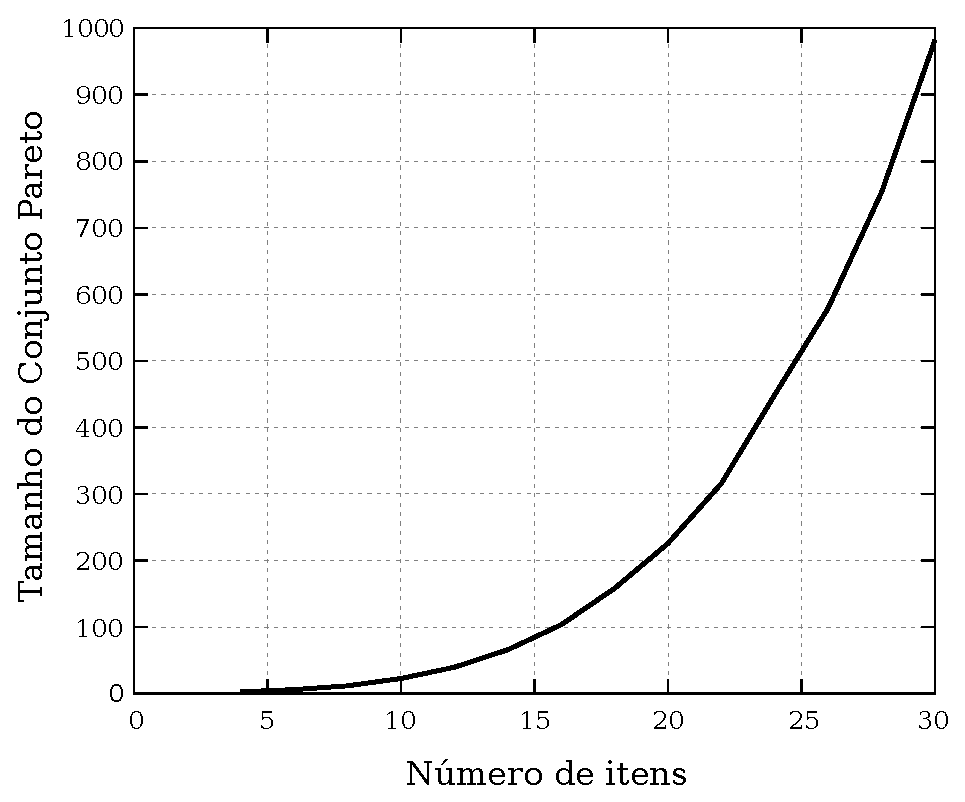
\includegraphics[scale=0.5]{img/mokp/par-grow-d3}
  \caption{Tamanho do \paretoset{} dado o tamanho da instância de problemas da mochila 3-objetivo.}
  \label{fig:pargrow3}
\end{figure}

Esse rápido crescimento tende a degradar a eficiência dos algoritmos,
uma vez que o processo de resolução do problema
deve gerar e manter uma grande quantidade de soluções,
especialmente em contextos exatos, nos quais é necessário a enumeração completa das soluções que compõem o \paretoset{}.
Este motivo tem levado pesquisadores a desenvolverem métodos heurísticos,
que buscam dar uma solução aproximada, demandando um menor esforço computacional~\cite{deb2002fast,zitzler1998multiobjective,zhang2007moea}.

\missingf{- a enumeração total das soluções remete a adoção de método força bruta. Acho que precisa reescrever isso.

\resp Para esclarecer, mudei: enumeração total das soluções exatas.).

- achei que nao ficou bom.
Nao seria melhor a enumeracao completa das soluçoes que compoem o conjunto pareto?
\resp Sim, ficou melhor. Alterei.

}

Outra alternativa viável, porém não trivial, de se reduzir o tempo computacional
demandado por um algoritmo é através da otimização de seus procedimentos,
como por exemplo, pela utilização de uma estrutura de dados mais adequada
para a operação, que pode reduzir o esforço computacional demandado pelo algoritmo
~\cite{cormen2009introduction, aho1974design,knuth1973fundamental}.

\section{Objetivo}

Este trabalho propõe a otimização dos procedimentos de manipulação do conjunto
de soluções, mais especificamente da operação de verificação de dominância de uma solução,
dado um conjunto de soluções, visto que esta operação é de grande
demanda tanto em contextos exatos quanto em contextos heurísticos.
Para isso, a operação de verificação de dominância é interpretada como
o problema de decidir se existe algum ponto em uma determinada região
do espaço multidimensional.

Esse tipo de problema, chamado \emph{busca de faixa}, é bem conhecido em alguns
ramos da computação, como na computação gráfica e desenvolvimento de jogos,
onde é necessário verificar a colisão entre pontos e polígonos~\cite{sedgewick1988algorithms}.
Visando a eficiência da operação, a busca de faixa é geralmente executada
com o auxílio de uma estrutura de indexação multidimensional,
das quais a \kdtree{} é uma das mais indicadas para este fim~\cite{agarwal1999geometric, sedgewick1988algorithms}.

O objetivo do presente trabalho é demonstrar que a utilização de estruturas
de indexação multidimensional, mais especificamente a \kdtree{}, pode aumentar a performance
de algoritmos para problemas da mochila multiobjetivo, mais especificamente em casos
que possuam conjuntos Paretos com grande quantidade de soluções, ao reduzir
o número total de avaliações de solução necessárias para a execução do algoritmo.
%deixando o algoritmoaté $2.3$ vezes mais rápido em casos bi-objetivo e até $15.5$ em casos 3-objetivo.
A eficácia da proposta será avaliada através de
testes computacionais, para os quais serão analisados o número de avaliações
de solução e o tempo computacional demandado pelos algoritmos em instâncias
consideradas pela literatura.

\missingf{- O objetivo é mostrar que kdtree é adequada para problemas multiobjetivo em geral ou especificamente
para mochila multiobjetivo? Isso precisa ficar bem claro!!! Se for o geral tem que justificar porque só experimenta
com mochila e que fazendo isso é razoável generalizar do específico para o geral. Me parece mais dificil!!!

\resp A proposta é otimizar para o problema da mochila.
Testar com outros problemas seria um trabalho futuro. Ajustei o texto.
}

\missingf{- Sua principal contribuição é a aplicacao de kd-tree para problemas (da mochila?) multiobjetivo em especial em casos
de problemas que possuem conjuntos Paretos com grande quantidade de soluções e problemas com mais de dois
objetivos...
Aqui vc precisa vender muito bem seu peixe!!!
Tem que dizer porque considera isso uma contribuição  significativa (para justificar um doutorado).
Tem trabalhos que fizeram algo semelhante, isto é, cujo objetivo é usar estruturas de dados para melhor o desempenho do mesmo problema (ou problema semelhante)?
Se sim,  tem que descrever, referenciar e dizer no que diferem da sua contribuiçao. Tem trabalhos nos quais o objetivo é usar
a kd-tree para melhorar o desempenho de algoritmos em problemas de otimizacao (multiobjetivo em geral ou da
mochila em geral)? Se sim, tem que descrever, referenciar e dizer no que diferem da sua contribuiçao.
}

Esta avaliação será feita no contexto exato
utilizando o algoritmo de Bazgan, considerado pela literatura
como o método exato mais eficiente para o problema~\cite{bazgan2009}.
No trabalho original do algoritmo, é proposta a utilização da árvore AVL
como estrutura de dados auxiliar para indexação de soluções em casos bi-objetivo,
sendo utilizada a lista encadeada para o caso 3-objetivo.
As respectivas estruturas de dados foram originalmente utilizadas,
provavelmente, diante do foco do trabalho, o qual é dedicado à proposta do algoritmo
e suas provas de corretude.
Diante disso, perdura a carência de uma maior investigação sobre a utilização de
estruturas de dados.

Para esta avaliação será utilizado um conjunto de 4 tipos de instâncias
por ser o conjunto proposto pela literatura para testes em abordagem exata
~\cite{bazgan2009,figueira2013algorithmic,correia2018},
contemplando tanto casos fáceis como difíceis do problema através da
exploração de diferentes características de instância.

A avaliação também será feita no contexto heurístico, por este ter uma demanda computacional diferente
da abordagem exata, não necessitando de enumerar todo o \paretoset{}, mas apenas uma aproximação deste.
Para a abordagem heurística será utilizada uma implementação da metaheurística
evolutiva chamada evolução estocástica por complexos (\emph{shuffled complex evolution} em inglês).
A evolução estocástica por complexos pretende ser uma metaheurística robusta,
que apresentou êxito em diversos problemas~\cite{duan1992effective, elbeltagi2007modified, zhao2015shuffled, bhattacharjee2014shuffled, baroni2015shuffled,baroni2016shuffled} porém,
ainda não havia sido aplicada ao problema da mochila multiobjetivo,
representando também uma contribuição do presente trabalho.

Para os testes computacionais no contexto heurístico,
serão consideradas as mesmas instâncias utilizadas pela literatura
para testar os principais algoritmos heurísticos
~\cite{zitzler1998multiobjective, deb2002fast,zhang2007moea,zouache2018cooperative}.
Em ambos os contextos serão observados tanto o tempo computacional quanto o número de avaliações de solução necessários
para a execução de cada algoritmo.


\missingf{
\begin{itemize}
\item{
- voce precisa destacar e descrever melhor a metodologia de pesquisa utilizada. Quais sao as instâncias
consideradas pela literatura (referenciar)? Quais sao as caracteristicas dessas instancias? Explicar porque as escolheu!
Porque vale a pena avaliar usando essas instancias? Elas são dificeis? O comportamento observado nelas pode ser
generalizado para o resto do universo (provavelmente não, mas a justificativa pode ser que é o que há de disponível).
Existem outras na literatura que vc não escolheu? Se existem, tem que explicar porque nao as escolheu...

\resp Ok, detalhei sobre isso no texto. }
\item{ Porque escolheu avaliar tanto no exato quanto no heuristico?

\resp Pois possuem demandas computacionais diferentes. Expliquei no texto. }

\item{ Tem que justificar melhor a escolha pelo algoritmo da  Bazgan...
Dizer que é o melhor da literatura apenas não é o suficiente... Tem referencia recente dizendo que ele é o melhor?
Se não tiver, vc deve mostrar quais seriam as opcoes (contemporaneas) e porque vc considera o da Bazgan o melhor.

\resp A referência é o próprio artigo da Bazgan que testa com os outros exatos propostos. Desde então nenhum outro artigo mostrou algum exato melhor.
Coloquei a referência.}

\item{ Qual a heuristica evolutiva escolheu e porque a escolheu? Porque nao escolheu a com melhores resultados na literatura?
(Sei que nao dá para colocar aqui a resposta real!!! Mas, é preciso tentar criar algum(ns) argumento(s) que defendam a
posicao adotada. Pode ser algo do tipo mais facil de ser implementada, precisar de menos tuning, exigir menos parametros ou
até um argumento mais fraco de que era uma heuristica nunca aplicada antes a mochila multiobjetivo (essa é fraca
porque com certeza tem varias metaheuristicas até mais populares que tb nao devem ter sido aplicadas ao problema).
Pense ai... Note que vc também está colocando como contribuição do trabalho... Tem que vender bem esse peixe tb!

\resp Expliquei que escolhi o SCE por ser aparentemente robusto, ter sido usado com sucesso em
outros problemas mas nunca aplicado ao MOKP. Também tentei deixar claro na tese que a aplicação
do SCE para um problema multiobjetivo não é direta, mas precisa de algumas adaptações, que também é
contribuição do trabalho.
}
\end{itemize}
}

\section{Histórico}

% Parágrafos
% - Inicio do trabalho se deu da pesquisa da EDP (apresentação do problema real)
% - Modelagem do problema real em problema da mochila multidimensional (apresenta o MKP)
% - Intenção de desenvolver um algoritmo para solução do problema, porém resolvedor exato muito bom
% - Apresentação do desempenho do resolvedor exato (gráfico de gap para instância difícil) não justificando desenvolvimento de outro algoritmo
% - Durante pesquisa, proposta de aceleração para algoritmo de programação dinâmica usando a kdtree
% - Kdtree acelera, porém não torna algoritmo exato competitivo no contexto do MKP, pois outros algoritmo são melhores, porém,
%     no contexto onde os vários estados devem ser obrigatoriamente enumerados, a kdtree deve ser eficiente

A proposta do presente trabalho surgiu após a execução de um projeto de pesquisa abordando
um problema real de otimização, levantado junto à EDP-Escelsa, empresa distribuidora de energia elétrica local.
%Entre suas atribuições, a Agência Nacional de Energia Elétrica (ANEEL) deve estimular a
%redução da energia perdida durante a distribuição.
Um dos mecanismos da Agência Nacional de Energia Elétrica (ANEEL) para estimular
a redução de perda de energia é a definição de metas,
que estipulam a quantidade máxima de energia perdida pela distribuidora por
causas não-técnicas. As distribuidoras, por sua vez, fazem seus planejamentos de forma a tentar
atingir esta meta, executando diversas ações de redução de perda,
respeitando orçamentos determinados, como orçamento de capital e orçamento de mão de obra.

Na ocasião, o plano de ações de redução de perda era selecionado manualmente por especialistas, buscando,
por tentativa e erro, escolher dentre um portfolio de ações, a combinação que obtém o melhor resultado, respeitando os orçamentos determinados.
Diante disso, a primeira etapa do projeto de pesquisa foi a modelagem do problema real
como um problema da mochila multidimensional~\cite{puchinger2010multidimensional}.
Apesar de também ser um problema de otimização escalar, o problema da mochila multidimensional
difere do problema da mochila clássico por possuir múltiplas restrições de capacidade, que no problema real em questão,
representa recursos como orçamento com capital, orçamento com mão de obra e quantidade máxima de execução das ações.
Sabendo-se que o problema da mochila multidimensional é \nphard{}, visou-se o desenvolvimento de uma heurística para a resolução do problema.

A forma ideal de se avaliar a qualidade da solução encontrada por uma heurística é comparando-a,
quando possível, com a solução exata ou, se não, com uma solução que possua alguma garantia de qualidade.
Diante disso, visando validar a qualidade das heurísticas desenvolvidas,
foi utilizado um resolvedor exato que implementa o algoritmo \emph{branch-and-cut}~\cite{padberg1991branch,mitchell2002branch} para obter as
soluções ótimas para o problema.

O algoritmo \emph{branch-and-cut} não só garante encontrar a solução ótima ao final da execução,
mas também apresenta uma garantia de qualidade da melhor solução encontrada no decorrer do processo.
Essa garantia é determinada através da estipulação de um limite superior para o
valor de objetivo do problema, o qual é gradativamente reduzido à medida que as soluções
do problema são enumeradas.
O algoritmo é encerrado quando o valor de limite superior coincide com o valor objetivo da
melhor solução encontrada.

Esse garantia de qualidade apresentada pelo algoritmo permite que o mesmo seja encerrado
antes de sua execução completa, caso a qualidade da melhor solução encontrada seja satisfatória.
De fato, em muitos casos, a solução exata do problema é encontrada em momentos iniciais do algoritmo, ficando a parte final da execução dedicada apenas à prova computacional
da otimalidade da solução encontrada.

Durante a execução do resolvedor, observou-se que, apesar do encerramento total do algoritmo
demandar horas, em poucos segundos alcançava-se uma solução com qualidade bem próxima à ótima.
A Tabela~\ref{tab:mkp} apresenta a progressão da qualidade da melhor solução encontrada pelo resolvedor
para uma das instâncias do problema considerada pela literatura como
uma das mais difíceis, possuindo 500 itens e 30 dimensões.
\begin{table}[ht]
  \centering
  The multidimensional knapsack problem (MKP) is a strongly NP-hard combinatorial
optimization problem which can be viewed as a resource allocation problem and
defined as follows:
\vspace{-15pt}
\begin{align*}
    \text{max} ~ & {\mymathstyle \sum_{j=1}^n p_j x_j} \\[3pt]
    \text{s. to} ~ & {\mymathstyle \sum_{j=1}^n w_{ij} x_j \leqslant c_i \quad i \in \{1, \ldots, m\}}\\
   & x_j \in \{0, 1\}, \quad j \in \{1, \ldots, n\}.
\end{align*}
\vspace{30pt}
The work address the application of a metaheuristic called
shuffled complex evolution (SCE) to the MKP.

  \caption{Progressão da qualidade da melhor a solução encontrada pelo resolvedor exato.}
  \label{tab:mkp}
\end{table}

Cada linha da Tabela~\ref{tab:mkp} registra o momento em que uma nova melhor solução foi encontrada
pelo resolvedor exato.
A primeira coluna apresenta o tempo total de execução (em segundos).
A segunda coluna apresenta a qualidade da melhor solução encontrada (em porcentagem) em relação ao limite superior computado.
Pode-se observar que em menos de 1 segundo o algoritmo foi capaz de encontrar uma solução com
qualidade mínima de $99.63\%$ do valor ótimo.
Fato semelhante pôde ser observado em todas as instâncias do problema,
o que resultou por enfraquecer a justificativa de desenvolvimento de uma heurística.
Diante disso, foi adotada como solução satisfatória a fornecida pelo resolvedor.

Contudo, durante a fase de pesquisa de algoritmo exatos, um dos algoritmos estudados
foi o algoritmo de Nemhauser e Ulmann~\cite{nemhauser1969discrete}
adaptado para o problema da mochila multidimensional.
O algoritmo de Nemhauser e Ulmann é um algoritmo de programação dinâmica que originalmente
computa a solução exata para o problema da mochila clássico.
Porém, com poucas adaptações, o algoritmo pode ser aplicado a algumas variações do problema clássivo, inclusive ao caso multidimensional.

Ao longo do processo de solução, o algoritmo de Nemhauser e Ulmann
manipula uma crescente quantidade de estados,
representando as possíveis soluções do problema.
Essa grande quantidade de estados resulta na degradação da performance do algoritmo.
Na tentativa de atenuar essa degradação, propôs-se a indexação multidimensional
dos estados utilizando a \kdtree{}, com o objetivo de acelerar sua manipulação.

A aplicação da proposta apresentou bons resultados, porém, diante do
desempenho do algoritmo \emph{branch-and-cut}, não pôde tornar o
algoritmo de programação dinâmica competitivo no contexto multidimensional.
Contudo, cogitou-se ser proveitosa a aplicação da proposta de indexação multidimensional
em contextos onde a enumeração dos estados gerados é estritamente necessária,
como o é no caso multiobjetivo.


\section{Estrutura da Tese}

A estrutura deste trabalho tem a seguinte organização.
O Capítulo~\ref{cap:mokp} aborda o problema da mochila multiobjetivo,
apresentando as abordagens exata e heurística que foram utilizadas no trabalho.
O Capítulo~\ref{cap:kdtree} apresenta a proposta de utilização da \kdtree\ como
estrutura auxiliar de aceleração para a resolução do problema.
No Capítulo~\ref{cap:exp} são descritos os experimentos computacionais.
No Capítulo~\ref{cap:concl} são apresentadas as conclusões e os  trabalhos futuros.

%\missingt{
%Falar do problema e das estratégias de solução escolhida.
%Contextualizar essas estratégias e situar minha contribuição;
%Deixar claro que minha proposta é o uso da estrutura,
%tanto no caso exato quanto no caso heurístico (nos devidos algoritmos).
%}

%%% Tópicos da introdução
% - Introdução à problemas multiobjetivos, citando MOKP. Dficuldade de contruir conjunto solução.
% - Ressaltar a importancia do problema (aplicações).
% - Propostas de métodos extados porém, não suporta instancias grande.
% - Propostas de métodos heurísticos.
% - Exclarecer que grande parte da dificuldade é devido ao grande conjunto
%     de soluções eficientes que existem. Lhe dar com essas soluções é muito custoso.
%     (Motivar a busca por melhorias na manipulação das soluções)
% - Introduzir a operação de busca por solução dominada e associar à busca de faixa.
%     Falar da proposta do trabalho é utilizar a kdtree para indexar as
%     soluções e auxiliar na manipulação, em especial na consulta de dominancia.
% - Dizer que o trabalho explica a proposta e a testa no contexo exato
%     utilizando um algoritmo estado da arte e também no contexto heurístico utilizando
%     a implementação da meta-geuristica SCE para o MOKP  (que é também uma
%     contribuição do trabalho). A performance do SCE é comparado com a
%     de outros algoritmos heurísticos.
%     obs.: Já citar que no caso exato a kdtree é comparada
%       com a AVL (no caso 2-objetivo) e com a lista (no caso 3-objetivo).
%       No caso heurístico a kdtree é comparada com a lista.
% - Falar brevemente sobre os resultados obtidos.
% - Dizer que a implementação do nosso algoritmo ficou lenta, porém não
%     refuta a proposta da indexação, pela corretude do algoritmo e estruturas utilizadaso,
%     e número de comparações (explicar)
% - Explicar a estrutura da tese.